\documentclass[pdflatex,sn-mathphys-num,iicol]{sn-jnl}

\usepackage{bookmark}
\usepackage{tabularx}
\usepackage{tikz}
\usetikzlibrary{shapes.geometric, shapes.misc, arrows.meta, positioning, calc}
\usepackage{graphicx}
\usepackage{amsmath,amssymb,amsfonts}
\usepackage{booktabs}

\raggedbottom

\begin{document}

\title[Which Shift Costs a CQT--CNN the Most]{Which Acoustic Shift Costs a CQT--CNN the Most? A Per-Seed Factorized Evaluation on Isolated Piano Chords}

\author*[1]{\fnm{Cikal} \sur{Gemintang Seya}}\email{cikalgemintangseya1@gmail.com}

\author[1]{\fnm{Jasman} \sur{Pardede}}\email{jasman@itenas.ac.id}

\affil*[1]{\orgdiv{Informatics}, \orgname{Institut Teknologi Nasional Bandung}, \orgaddress{\street{Neglasari}, \city{Bandung}, \postcode{40124}, \state{West Java}, \country{Indonesia}}}

\abstract{Isolated piano-chord audio is a 36-class recognition problem, 12 roots crossed with three interval templates (major, minor, diminished). We train a compact Convolutional Neural Network (CNN) on Constant-Q Transform (CQT) features from a Techno T-9890i digital keyboard and evaluate it without fine-tuning under two recorded factors, first a recording-setting shift where the same keyboard is captured on three other microphones, then a keyboard shift where a Yamaha PSR-S910 is captured on two of those same recording settings, and finally under eval-only overlays. The architecture is retrained ten times, five seeds on the full 7{,}200-clip training set (\texttt{orig}) and five more after dropping sixteen silent clips (\texttt{clean}). In-domain accuracy stays at or above 0.999 for every run, which this training protocol makes closer to a memorization check than a difficulty measurement. Out of domain, the Techno-minus-Yamaha gap on a fixed recording setting is positive on all twenty matched checkpoints (sign test $p\approx10^{-6}$), and the keyboard costs more than the recording setting on 18 of the 20, both exceptions falling on the ROG Flow pair. Eval-only ESC-50 noise compounds the keyboard cost, while a measured microphone impulse response costs nothing, so synthetic recording-setting augmentation does not reproduce a recorded microphone change. Dropping the silent clips does not uniformly raise out-of-domain accuracy, since \texttt{clean} seed 42 falls to 0.348 / 0.368 on the two Yamaha datasets while the same-seed \texttt{orig} run holds 0.963 / 0.961. One seed can invert the apparent value of the data-quality fix and move the keyboard gap by tens of points, so we report every seed.}

\keywords{Constant-Q Transform, Convolutional Neural Network, domain shift, ablation, seed variance}

\maketitle

\section{Introduction}\label{sec_introduction}

Recognizing musical chords directly from raw audio is a foundational task in music information retrieval (MIR), underpinning automatic transcription, interactive music education, and real-time performance feedback \cite{Telila2023}. Unlike symbolic recognition, it must contend with sound production, since a chord played on one instrument, in one room, captured by one microphone does not produce the waveform of the same chord on a different instrument, room, and microphone \cite{Kusaka2024}.

That mismatch is acoustic domain shift, a change in the recorded signal rather than a claim that the instruments are acoustic pianos, and at least three factors drive it. Keyboard variation is the first, where another instrument's voice synthesis displaces chord vectors in feature space. Environmental shift is the second, where ambient noise and room acoustics absent from training move the scene. Recording-setting shift is the third, where a different microphone, its placement, and its on-device signal chain change the captured spectrum \cite{Kusaka2024,Majchrzak2025}. A classifier that latched onto a condition-specific cue instead of the interval structure pays for it out of domain \cite{Geirhos2020}. A joint shift matches deployment, but one number hides the cause, since a phone microphone on the Techno T-9890i and the Yamaha PSR-S910 on a laptop microphone already used for a recording-setting test are different problems, and neither is a noisy environment. Ranking the factors needs independently recorded datasets for each, plus a controlled synthetic overlay for the environment.

Time-frequency matrices classified with convolutional architectures dominate audio recognition \cite{Wolf-Monheim2025}, and chord recognition has used them since the first frame-level CNN acoustic models \cite{Korzeniowski2016}. The Constant-Q Transform (CQT) suits keyboard audio because, unlike the Short-Time Fourier Transform's linear bins, its bins are logarithmically spaced at a constant quality factor and align with semitones \cite{Lacoste2007}, so a transposition is a vertical shift and harmonic intervals keep a consistent shape \cite{Li2021}. Li \cite{Li2021} reported 84.2\% accuracy for CQT chord recognition against 75.3\% for STFT and 80.8\% for CENS chromagrams under one CNN, and Telila et al.\ \cite{Telila2023} report comparable gains. We keep CQT as the input. The 36 classes formed by 12 chromatic roots and 3 qualities demand fine-grained discrimination, since major and minor triads differ by a semitone in the third and diminished triads differ by a further semitone in the fifth \cite{Harte2010}. Convolutional kernels respond to small time-frequency neighborhoods \cite{Purwono2022}, so local interval geometry can in principle survive the envelope shift a new microphone or piano voice imposes.

Edwards et al.\ \cite{Edwards2024} run the closest controlled piano out-of-domain study, though on note-level transcription rather than chords. They replay MAESTRO MIDI on a Yamaha Disklavier in a studio, evaluate on MAPS, and degrade test audio with noise, EQ, pitch shift, and reverb. A studio-only model overfits that environment, and train-time mixing then recovers 88.4 MAPS note-onset F1 with no MAPS training audio. Kusaka and Maezawa \cite{Kusaka2024} use a related recipe for mobile transcription. Both treat augmentation as a training intervention, whereas we keep the opposite protocol, a clean-trained CQT--CNN with recorded and synthetic shifts only at evaluation, so each factor's cost is visible before anyone mixes the training set. Their pianos are acoustic and ours are digital, so the keyboard factor here is sample set, loudspeaker, and cabinet.

Chord papers still grow the vocabulary \cite{Majchrzak2025} or swap in conformers \cite{Akram2025}, test in-domain, and patch out-of-domain conditions with synthetic audio \cite{Byambatsogt2020,Ostermann2023}. Isolated piano chords lack a factorized reading of a CQT--CNN that also asks whether a training-set defect changes the ranking, and sixteen digital-silence clips sitting in the Techno training set, 8\% of one class, raise exactly that question. In-domain accuracy saturates at 1.00 and cannot answer it. Since a single-run benchmark hides exactly this kind of spread \cite{Bouthillier2021}, we retrain the architecture ten times, five seeds with the silent clips (\texttt{orig}) and five without (\texttt{clean}), and report every seed on every held-out condition.

This paper makes four contributions.
\begin{enumerate}
\item \textbf{A corpus recorded to separate the factors.} A Techno T-9890i training set with five held-out datasets: three recording-setting-shift datasets on that same keyboard, one of which (\texttt{vivo}) has no keyboard counterpart, and two Yamaha PSR-S910 keyboard-shift datasets captured on recording settings already used for the recording-setting tests.
\item \textbf{A shared representation and a repeated retrain.} One CQT feature format ($216\times188\times1$) into a compact CNN, retrained under two training-set configurations and five seeds on a single pinned GPU with deterministic kernels.
\item \textbf{A frozen-weight evaluation protocol.} Recording-setting change is tested apart from keyboard change with no fine-tuning, and eval-only noise, room, and microphone overlays are then applied on top, every seed reported.
\item \textbf{A per-seed ranking of the factors.} The recorded factors are ordered against each other and against the synthetic overlays, and the ablation of sixteen silent training clips asks whether a data-quality fix changes that order.
\end{enumerate}

\section{Methodology}\label{sec_methodology}

Fig.~\ref{fig_methodology} shows the pipeline, running from dataset acquisition through CQT extraction, the \texttt{orig}/\texttt{clean} $\times$ 5-seed CNN retrain, recorded out-of-domain evaluation, and eval-only overlays. The software stack is Python 3.10, TensorFlow 2.15, scikit-learn 1.7.2, Librosa 0.11.0, NumPy 1.26.4, and Matplotlib 3.10.8.

\begin{figure}[htbp]
  \centering
  \resizebox{0.92\columnwidth}{!}{%
  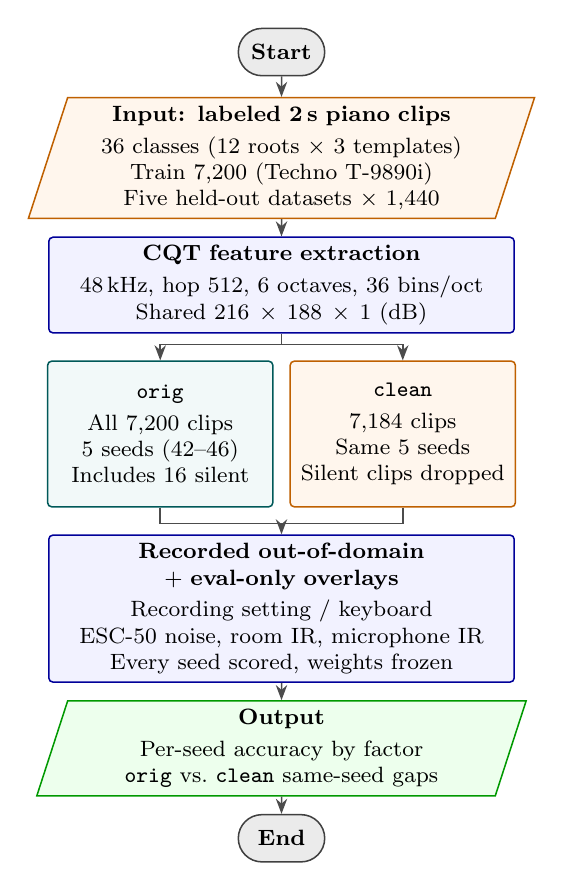
\begin{tikzpicture}[
    node distance=0.16cm and 0.10cm,
    >={Stealth},
    font=\footnotesize,
    base/.style={draw, align=center, minimum height=0.52cm, line width=0.55pt, inner sep=3pt},
    terminal/.style={base, shape=rounded rectangle, rounded rectangle arc length=180, draw=black!75, fill=black!8, minimum height=0.60cm, minimum width=1.8cm, inner xsep=10pt, inner ysep=2pt, font=\footnotesize\bfseries},
    process/.style={base, rectangle, rounded corners=1.5pt, draw=blue!60!black, fill=blue!5, text width=5.7cm},
    orig/.style={base, rectangle, rounded corners=1.5pt, draw=teal!70!black, fill=teal!5, text width=2.65cm, minimum height=1.85cm},
    clean/.style={base, rectangle, rounded corners=1.5pt, draw=orange!75!black, fill=orange!7, text width=2.65cm, minimum height=1.85cm},
    io/.style={base, trapezium, trapezium left angle=72, trapezium right angle=108, trapezium stretches body=true, draw=orange!75!black, fill=orange!7, text width=5.15cm, inner xsep=4pt},
    result/.style={base, trapezium, trapezium left angle=72, trapezium right angle=108, trapezium stretches body=true, draw=green!60!black, fill=green!7, text width=5.15cm, inner xsep=4pt},
    arrow/.style={->, line width=0.55pt, black!70}
  ]
    \node[terminal] (start) {Start};
    \node[io, below=0.26cm of start] (in1)
    {\textbf{Input: labeled 2\,s piano clips}\\[2pt]
     36 classes (12 roots $\times$ 3 templates)\\
     Train 7{,}200 (Techno T-9890i)\\
     Five held-out datasets $\times$ 1{,}440};
    \node[process, below=0.22cm of in1] (p2)
    {\textbf{CQT feature extraction}\\[2pt]
     48\,kHz, hop 512, 6 octaves, 36 bins/oct\\
     Shared $216 \times 188 \times 1$ (dB)};
    \node[orig, below left=0.34cm and 0.10cm of p2.south, anchor=north east] (o1)
    {\textbf{\texttt{orig}}\\[2pt]
     All 7{,}200 clips\\
     5 seeds (42--46)\\
     Includes 16 silent};
    \node[clean, below right=0.34cm and 0.10cm of p2.south, anchor=north west] (c1)
    {\textbf{\texttt{clean}}\\[2pt]
     7{,}184 clips\\
     Same 5 seeds\\
     Silent clips dropped};
    \node[process, below=0.34cm of $(o1.south)!0.5!(c1.south)$, anchor=north] (p5)
    {\textbf{Recorded out-of-domain $+$ eval-only overlays}\\[2pt]
     Recording setting / keyboard\\
     ESC-50 noise, room IR, microphone IR\\
     Every seed scored, weights frozen};
    \node[result, below=0.22cm of p5] (out)
    {\textbf{Output}\\[2pt]
     Per-seed accuracy by factor\\
     \texttt{orig} vs.\ \texttt{clean} same-seed gaps};
    \node[terminal, below=0.22cm of out] (endn) {End};
    \draw[arrow] (start) -- (in1);
    \draw[arrow] (in1) -- (p2);
    \draw[arrow] (p2.south) -- ++(0,-0.14) -| (o1.north);
    \draw[arrow] (p2.south) -- ++(0,-0.14) -| (c1.north);
    \coordinate (merge) at ($(p5.north)+(0,0.14)$);
    \draw[line width=0.55pt, black!70] (o1.south) |- (merge);
    \draw[line width=0.55pt, black!70] (c1.south) |- (merge);
    \draw[arrow] (merge) -- (p5.north);
    \draw[arrow] (p5) -- (out);
    \draw[arrow] (out) -- (endn);
  \end{tikzpicture}%
  }
  \caption{Experimental pipeline. Shared CQT features feed two training-set variants $\times$ five seeds. Eval-only overlays hit the five held-out datasets; CNN weights stay frozen after training.}
  \label{fig_methodology}
\end{figure}

\subsection{Two evaluation scenarios}\label{subsec_scenarios}

Scenario~1 (in-domain) holds instrument, environment, and recording setting fixed and asks whether the CQT space separates the 36 classes at all. Five-fold cross-validation on the 7{,}200 Techno takes measures this for the reference architecture, 80/20 per fold, with each fold retrained from a fresh initialization and a fixed per-fold seed, and each retrain below also reports its own held-out Techno test split.

Scenario~2 changes one factor at a time and tests each trained checkpoint with no fine-tuning. Three recording-setting-shift datasets keep the Techno T-9890i and change microphone, placement, and on-device signal chain (ThinkPad P14s internal mic, Vivo Y27s, ROG Flow X13 internal mic). Laptop and phone capture paths commonly apply automatic gain control and noise suppression that neither device logs, so this factor bundles transducer, codec, and unrecorded processing rather than isolating a frequency response. Two keyboard-shift datasets swap the instrument to a Yamaha PSR-S910 while reusing the ThinkPad and Flow recording settings already measured on the Techno, so \texttt{thinkpad} versus \texttt{thinkpad-2} and \texttt{flow} versus \texttt{flow-2} differ by keyboard alone. \texttt{vivo} has no Yamaha counterpart. Table~\ref{tab_datasets} lists all six datasets, and eval-only overlays (Section~\ref{subsec_noise}) hit the five held-out ones.

\begin{table*}[t]
\caption{Recorded datasets. The CNN is trained on \texttt{training} and evaluated on every row. $^\dagger$\texttt{vivo} has no Yamaha counterpart.}\label{tab_datasets}
\begin{tabular*}{\textwidth}{@{\extracolsep{\fill}}lllll@{}}
\toprule
Dataset & $N$ & Primary shift & Instrument & Recording setting \\
\midrule
\texttt{training} & 7{,}200 & None (in-domain) & Techno T-9890i & Redmi Pad 2 \\
\texttt{thinkpad} & 1{,}440 & Recording setting & Techno T-9890i & ThinkPad P14s \\
\texttt{vivo} & 1{,}440 & Recording setting$^\dagger$ & Techno T-9890i & Vivo Y27s \\
\texttt{flow} & 1{,}440 & Recording setting & Techno T-9890i & ROG Flow X13 \\
\texttt{thinkpad-2} & 1{,}440 & Keyboard & Yamaha PSR-S910 & ThinkPad P14s \\
\texttt{flow-2} & 1{,}440 & Keyboard & Yamaha PSR-S910 & ROG Flow X13 \\
\bottomrule
\end{tabular*}
\end{table*}

\subsection{Dataset acquisition}\label{subsec_acquisition}

A web recorder sends simultaneous MIDI note-on events over USB and captures the microphone. That removes manual playing errors and keeps each keyboard's loudspeaker, cabinet, and synthesis. Every dataset uses the same trigger list and voicing, so class identity does not change with the acoustic condition.

Each of the 36 classes is a three-note piano sound, one of 12 roots (C, C$\sharp$, \ldots, B) crossed with one of three interval templates (maj $+4,+3$; min $+3,+4$; dim $+3,+3$ semitones). A semitone occupies three CQT bins. Figures write \emph{C maj} and \emph{E dim}, while file names keep the fourth-octave suffix. All takes sit in that octave, inside C1--C7 (32.70--2{,}093\,Hz) \cite{Telila2023,Harte2010}. The dim template packs its three notes closer together than maj or min \cite{Byambatsogt2020}. The Techno T-9890i is a consumer arranger keyboard and the Yamaha PSR-S910 a workstation arranger, and both are digital instruments on a grand-piano preset that differ in sample set, loudspeaker, and cabinet.

The training set holds 200 samples per class, 7{,}200 total, from the Techno on an Acoustic Grand preset into a Redmi Pad 2 microphone, written as OGG/OPUS at 48{,}000\,Hz, 32-bit, mono, unfiltered, with attack delays of 0--150\,ms approximating keystroke asynchrony \cite{Bella2011}. Sixteen of those clips, 8\% of $C$ diminished and a recorder fault, are digital silence, and Section~\ref{subsec_ablation} trains with and without them. Each held-out dataset holds 40 takes per class, 1{,}440 in all, written as WAV. No evaluation clip enters training, validation, early stopping, or hyperparameter choice.

\subsection{CQT feature extraction}\label{subsec_cqt}

We compute CQT with \texttt{librosa.cqt()}. Each bin $f_k$ has constant quality
\begin{equation}
Q = \frac{f_k}{f_{k+1} - f_k} = \frac{1}{2^{1/B} - 1}
\label{eq_cqt}
\end{equation}
where $B$ is bins per octave \cite{Li2021,Lacoste2007}. Logarithmic spacing lines bins up with semitones, so a major third is the same bin distance on every root \cite{Harte2010}.

Analysis runs at 48\,kHz with hop 512, a Hann window, and 6 octaves at 36 bins per octave, covering C1 (32.70\,Hz) to C7 (2{,}093\,Hz) in 216 bins. Three bins per semitone resolve the three interval templates \cite{Akram2025}. Each clip is truncated to a fixed 2.0\,s, so Equation~\ref{eq_frames} gives $2.0\times 48000/512=187.5$, and the stored CQT rounds up to 188 frames with shape $216 \times 188 \times 1$. Magnitudes go to dB with Librosa \texttt{amplitude\_to\_db} (\texttt{ref=max}). Training, every recorded dataset, and every overlay share these parameters.

\begin{equation}
\text{frames} = \frac{\text{duration} \times \text{sample rate}}{\text{hop size}}
\label{eq_frames}
\end{equation}

\begin{figure}[htbp]
\centering
\includegraphics[width=\columnwidth]{fig-cqt-train.png}
\caption{Training CQT of C maj ($+4,+3$) and C min ($+3,+4$): same root, one-semitone gap in the middle note. Frequency in Hz.}
\label{fig_cqt}
\end{figure}

\subsection{CNN architecture and training}\label{subsec_cnn}

The CNN follows Wolf-Monheim \cite{Wolf-Monheim2025}, originally designed for environmental sound classification on ESC-50. Its compact four-block convolutional structure without recurrent layers or attention suits fixed-window classification from static spectrograms.

Table~\ref{tab_cnn_arch} lists layers. The input batch-normalization layer runs on the frequency axis, fitting one scale and shift per CQT bin to the Techno training distribution and applying that fixed 216-parameter transform to every clip at inference. The four Conv2D--MaxPooling2D blocks build a hierarchy that moves from 64 filters for low-level spectral texture to 128 for mid-level interval patterns and then two blocks of 256 for chord-quality abstractions. A single $3\times3$ kernel spans one semitone at 3 bins per semitone, narrower than the maj/min/dim contrast, so quality discrimination accumulates across blocks as pooling widens the effective receptive field \cite{Purwono2022}. Flatten feeds 36{,}608 units into a 256-unit dense layer, about 9.4\,M of the model's parameters, and that layer reads absolute time-frequency position. Apart from dropout at the head the design carries no regularization, with no weight decay and no train-time augmentation.

\begin{table}[t]
\caption{CNN architecture specification}\label{tab_cnn_arch}
\begin{tabularx}{\columnwidth}{@{}lXl@{}}
\toprule
Layer & Output shape & Notes \\
\midrule
BatchNorm & $216{\times}188{\times}1$ & Per frequency bin \\
Conv2D & $216{\times}188{\times}64$ & $3{\times}3$, ReLU, same \\
MaxPool & $108{\times}94{\times}64$ & $2{\times}2$, stride 2 \\
Conv2D & $108{\times}94{\times}128$ & $3{\times}3$, ReLU, same \\
MaxPool & $54{\times}47{\times}128$ & $2{\times}2$, stride 2 \\
Conv2D & $54{\times}47{\times}256$ & $3{\times}3$, ReLU, same \\
MaxPool & $27{\times}23{\times}256$ & $2{\times}2$, stride 2 \\
Conv2D & $27{\times}23{\times}256$ & $3{\times}3$, ReLU, same \\
MaxPool & $13{\times}11{\times}256$ & $2{\times}2$, stride 2 \\
Flatten & 36{,}608 & --- \\
Dense & 256 & ReLU \\
Dropout & 256 & rate 0.5 \\
Dense & 36 & Softmax \\
\bottomrule
\end{tabularx}
\end{table}

Training follows Table~\ref{tab_cnn_train}. A stratified 90/10 split holds out the test partition, and Keras then reserves the last 10\% of the training partition for validation without re-stratifying it, giving 81/9/10 overall. The seed sets that split, the weight initialization, and the Python, NumPy, and TensorFlow global RNGs, so a seed here indexes a bundle of split and initialization rather than initialization alone. \texttt{ReduceLROnPlateau} multiplies the learning rate by 0.1 after 2 stagnant validation-loss epochs, \texttt{EarlyStopping} stops after 6 and restores the best-validation-loss weights, and training runs for a maximum of 50 epochs \cite{Wolf-Monheim2025}. Every one of the ten retrains ran as an isolated OS process on the same pinned RTX 2080 Ti with \texttt{TF\_DETERMINISTIC\_OPS=1} and batch size 32, so the seed-to-seed spread below is not kernel-selection noise across devices. Feature extraction and evaluation used a ROG Flow X13 (Ryzen 7 6800HS, 16\,GB RAM) and Google Colaboratory (T4/A100).

\begin{table}[t]
\caption{CNN training configuration}\label{tab_cnn_train}
\begin{tabular}{@{}ll@{}}
\toprule
Parameter & Value \\
\midrule
Seeds & 42, 43, 44, 45, 46 \\
Train / Val / Test split & 81\% / 9\% / 10\% \\
Batch size & 32 \\
Initial learning rate & 0.001 \\
Optimizer & Adam \\
Weight initialization & Glorot uniform \\
Loss & Categorical cross-entropy \\
Max epochs & 50 \\
EarlyStopping & patience 6, restore best \\
ReduceLROnPlateau & factor 0.1, patience 2 \\
\bottomrule
\end{tabular}
\end{table}

\subsection{Training-set ablation}\label{subsec_ablation}

Two training configurations share Table~\ref{tab_cnn_arch} and Table~\ref{tab_cnn_train}. \texttt{orig} uses all 7{,}200 clips, including the sixteen silent $C$ diminished takes, while \texttt{clean} drops those sixteen (7{,}184 remaining) and changes no hyperparameter. Each is retrained from seeds 42--46, producing ten checkpoints.

The two variants are not a paired ablation in the strict sense. The seed generates the split from whichever pool it is handed, so \texttt{orig} seed 42 and \texttt{clean} seed 42 draw different train/validation/test partitions as well as different initializations, and the seed value is the only quantity they share. Same-seed comparisons below therefore measure dropping the clips and redrawing the split together. Deleting the silent clips from inside a fixed partition would separate the two, but that run is not in this report.

\subsection{Eval-only overlays}\label{subsec_noise}

Three overlays hit the already out-of-domain datasets without retraining, applied to all ten checkpoints with overlay probability 1, a fixed draw seed, and no write-back into training.

\emph{Noise.} 400 ESC-50 clips over 10 interior and domestic classes \cite{Piczak2015} become CQT matrices under the same hop and binning as the chord features. Mixing happens in the CQT power domain: for a chord magnitude matrix $X$ and a time-rolled noise matrix $N$,
\begin{equation}
Y = \sqrt{X^{2} + \alpha^{2} N^{2}}, \quad
\alpha^{2} = \frac{\overline{X^{2}}}{\overline{N^{2}}\,10^{\,\mathrm{SNR}/10}} ,
\label{eq_mix}
\end{equation}
where the bars are means over the full $216\times188$ plane, so SNR is broadband and per clip, drawn uniformly from $[10,25]$\,dB. Power-domain mixing omits phase interaction and any interaction with the capture chain, so this is a controlled interior overlay rather than a claim that ESC-50 matches a recorded environment.

\emph{Room and microphone impulse responses.} These convolve the evaluation waveform before CQT extraction, one response drawn per clip. The room bank holds 174 indoor responses from the IR Survey \cite{Traer2016} with bathrooms and outdoor spaces removed, and the microphone bank holds six measured vintage-capsule responses. Both are resampled to 48\,kHz and leading-silence trimmed.

\subsection{Evaluation metrics}\label{subsec_metrics}

Accuracy is the fraction of clips with the correct label, and macro precision, recall, and F1 are unweighted means of the usual one-versus-rest quantities over the 36 classes. Tables report accuracy per seed. A \emph{keyboard gap} is the recording-setting accuracy minus the matched keyboard-shift accuracy on the same checkpoint, \texttt{thinkpad} minus \texttt{thinkpad-2} or \texttt{flow} minus \texttt{flow-2}, and an \emph{overlay tax} is recorded accuracy minus overlay accuracy on the same checkpoint and dataset. Both are in accuracy points. At $n=1{,}440$ a 95\% Wald interval on an accuracy near 0.90 spans $\pm1.6$ points and near 0.80 spans $\pm2.1$, so differences below roughly 3 points between two cells are not resolved by these datasets.

\section{Results}\label{sec_results}

\subsection{In-domain performance}\label{subsec_res_indomain}

Every clip becomes a $216 \times 188$ CQT dB matrix, and Fig.~\ref{fig_cqt} shows C maj and C min from the training set, the same root but one semitone apart in the middle note. Under Scenario~1 the CNN scores 1.00 accuracy, precision, recall, and F1 on every fold of the 7{,}200 Techno takes. On the held-out Techno test split of the ten retrains, every \texttt{orig} seed reaches 1.000, and so do \texttt{clean} seeds 42, 44, 45, and 46, with seed 43 close behind at 0.999. Resubstitution on the full training dataset reaches 0.9999, with one $C$ diminished clip predicted as $C$ minor.

That saturation says less than it appears to. The 200 takes of a class share one keyboard, one preset, one fourth-octave voicing, and one MIDI trigger list, differing only by an attack delay of 0--150\,ms, so a random split places near-copies of each test clip in the training partition. In-domain 1.00 is close to a memorization check, and the 5-fold run measures the same near-degeneracy a second time. What this paper can answer is how far that memorizer transfers, which is Scenario~2.

\subsection{Recorded out-of-domain accuracy}\label{subsec_res_recorded}

Table~\ref{tab_seeds} lists accuracy for each seed, grouped by recording setting. Recording-setting means stay close under both variants, 0.961 / 0.903 / 0.911 on \texttt{orig} against 0.962 / 0.894 / 0.900 on \texttt{clean} for \texttt{thinkpad}, \texttt{vivo}, and \texttt{flow}. The keyboard means separate them, 0.803 and 0.815 on \texttt{orig} against 0.719 and 0.728 on \texttt{clean}, and that drop traces to one seed. \texttt{clean} seed 42 scores 0.348 and 0.368 on the two Yamaha sets while holding 0.985 / 0.884 / 0.831 on Techno. No other \texttt{clean} seed repeats it, and seed 43, the weakest recording-setting run at 0.857 / 0.742 / 0.810, is not the weakest keyboard run. On \texttt{orig} the spread is narrower, running from seed 42 at 0.963 / 0.961 on Yamaha down to seed 45 at 0.705 / 0.740.

Dropping the silent clips therefore does not produce a uniformly better out-of-domain model. Against the \texttt{orig} run of the same seed, \texttt{clean} is better on some cells, seed 45 on every dataset and seed 44 on four of five, and worse on others, seed 42 on every dataset and seed 43 on four of five. Section~\ref{subsec_ablation} bars reading any single cell as the effect of the sixteen clips on their own.

\begin{table*}[t]
\caption{Out-of-domain accuracy by seed and recording setting, recorded (top) and under eval-only ESC-50 interior noise (bottom). Gap is Techno minus Yamaha on the same checkpoint, in accuracy points computed before rounding, so it can differ from the printed columns by 0.1; an overlay tax is a recorded cell minus its noise cell. \texttt{orig} keeps all 7{,}200 clips, \texttt{clean} drops sixteen silent ones. \texttt{vivo} has no Yamaha pair. $^\dagger$One-seed collapse, not the variant.}\label{tab_seeds}
\setlength{\tabcolsep}{3.5pt}
\begin{tabular*}{\textwidth}{@{\extracolsep{\fill}}llccccccc@{}}
\toprule
& & \multicolumn{3}{c}{ThinkPad} & \multicolumn{3}{c}{Flow} & Vivo \\
\cmidrule(lr){3-5} \cmidrule(lr){6-8}
Variant & Seed & Techno & Yamaha & Gap & Techno & Yamaha & Gap & Techno \\
\midrule
\multicolumn{9}{@{}l}{\textit{Recorded}} \\
\texttt{orig} & 42 & 0.999 & 0.963 & 3.6 & 0.994 & 0.961 & 3.3 & 0.999 \\
\texttt{orig} & 43 & 0.967 & 0.719 & 24.8 & 0.863 & 0.720 & 14.2 & 0.896 \\
\texttt{orig} & 44 & 0.958 & 0.847 & 11.1 & 0.940 & 0.842 & 9.8 & 0.883 \\
\texttt{orig} & 45 & 0.895 & 0.705 & 19.0 & 0.801 & 0.740 & 6.0 & 0.776 \\
\texttt{orig} & 46 & 0.984 & 0.780 & 20.4 & 0.958 & 0.810 & 14.7 & 0.960 \\
\texttt{orig} & Mean & 0.961 & 0.803 & 15.8 & 0.911 & 0.815 & 9.6 & 0.903 \\
\texttt{clean} & 42 & 0.985 & 0.348$^\dagger$ & 63.8 & 0.831 & 0.368$^\dagger$ & 46.3 & 0.884 \\
\texttt{clean} & 43 & 0.857 & 0.698 & 15.9 & 0.810 & 0.685 & 12.6 & 0.742 \\
\texttt{clean} & 44 & 0.975 & 0.925 & 5.0 & 0.981 & 0.935 & 4.7 & 0.971 \\
\texttt{clean} & 45 & 0.999 & 0.884 & 11.5 & 0.988 & 0.903 & 8.5 & 0.997 \\
\texttt{clean} & 46 & 0.996 & 0.740 & 25.6 & 0.891 & 0.749 & 14.2 & 0.879 \\
\texttt{clean} & Mean & 0.962 & 0.719 & 24.3 & 0.900 & 0.728 & 17.3 & 0.894 \\
\midrule
\multicolumn{9}{@{}l}{\textit{Eval-only ESC-50 noise}} \\
\texttt{orig} & 42 & 0.958 & 0.924 & 3.4 & 0.948 & 0.922 & 2.6 & 0.949 \\
\texttt{orig} & 43 & 0.832 & 0.506 & 32.6 & 0.792 & 0.526 & 26.5 & 0.802 \\
\texttt{orig} & 44 & 0.864 & 0.689 & 17.5 & 0.869 & 0.700 & 16.9 & 0.836 \\
\texttt{orig} & 45 & 0.749 & 0.469 & 28.0 & 0.749 & 0.501 & 24.7 & 0.688 \\
\texttt{orig} & 46 & 0.888 & 0.661 & 22.7 & 0.873 & 0.699 & 17.4 & 0.860 \\
\texttt{orig} & Mean & 0.858 & 0.650 & 20.8 & 0.846 & 0.670 & 17.6 & 0.827 \\
\texttt{clean} & 42 & 0.808 & 0.258$^\dagger$ & 55.0 & 0.682 & 0.261$^\dagger$ & 42.1 & 0.724 \\
\texttt{clean} & 43 & 0.753 & 0.522 & 23.1 & 0.738 & 0.517 & 22.1 & 0.669 \\
\texttt{clean} & 44 & 0.953 & 0.866 & 8.7 & 0.933 & 0.873 & 6.0 & 0.924 \\
\texttt{clean} & 45 & 0.958 & 0.829 & 12.9 & 0.948 & 0.835 & 11.3 & 0.935 \\
\texttt{clean} & 46 & 0.906 & 0.594 & 31.2 & 0.837 & 0.626 & 21.1 & 0.794 \\
\texttt{clean} & Mean & 0.876 & 0.614 & 26.2 & 0.828 & 0.622 & 20.5 & 0.809 \\
\bottomrule
\end{tabular*}
\end{table*}

\subsection{Ranking the recorded factors}\label{subsec_res_factors}

Table~\ref{tab_seeds} isolates the keyboard with the two matched-pair gaps. All twenty checkpoint--pair combinations lose accuracy when the keyboard changes and the recording setting does not. The gap is never zero and never negative, which a sign test puts at $p\approx10^{-6}$, and sixteen of the twenty exceed the $\pm3$-point resolution of Section~\ref{subsec_metrics}. Its size is another matter, since on \texttt{orig} the ThinkPad gap runs from 3.6 to 24.8 points across five seeds, and on \texttt{clean} it runs from 5.0 to 63.8.

Ranking the two recorded factors against each other needs a common baseline. Reading recording-setting cost as $1.000$ minus the Techno out-of-domain accuracy, and keyboard cost as the matched gap on the same checkpoint, the keyboard turns out to be the more expensive factor on 18 of the 20 comparisons. Both exceptions fall on the Flow pair. \texttt{orig} seed 45 pays 19.9 points for the recording setting against 6.0 for the keyboard, and \texttt{clean} seed 43 pays 19.0 against 12.6. Two further comparisons sit inside the resolution limit and are unordered, \texttt{orig} seed 43 on Flow at 13.7 against 14.2, and \texttt{clean} seed 43 on ThinkPad at 14.3 against 15.9. Both inverting seeds carry an unusually weak Techno baseline on Flow, the same instability the per-seed report exists to expose. Averaged over seeds and datasets, the recording setting costs 7.5 points on \texttt{orig} and 8.1 on \texttt{clean}, against mean keyboard gaps of 9.6--15.8 and 17.3--24.3.

\subsection{Where the keyboard error lands}\label{subsec_res_quality}

Averaged over the five seeds, the three qualities separate under keyboard shift. On \texttt{orig} the recall of major, minor, and diminished triads is 0.989 / 0.930 / 0.963 on \texttt{thinkpad} against 0.835 / 0.843 / 0.730 on \texttt{thinkpad-2}, and 0.954 / 0.897 / 0.882 on \texttt{flow} against 0.827 / 0.857 / 0.760 on \texttt{flow-2}. \texttt{clean} repeats the pattern lower, diminished falling to 0.639 and 0.648 on the two Yamaha sets. The $+3,+3$ template packs its notes closest together, and it is the first quality the model loses when the instrument changes, since it already suffers most under a recording-setting change alone (0.827 on \texttt{vivo} against 0.978 for major).

\subsection{Eval-only overlays}\label{subsec_res_noise}

The lower half of Table~\ref{tab_seeds} lists accuracy after ESC-50 interior noise is mixed into every evaluation clip. Room and microphone impulse responses were collected under the same protocol.

Noise lowers accuracy on all 50 dataset--seed cells of both variants. On \texttt{orig} the mean tax runs 10.2, 7.6, and 6.5 points on the three Techno sets and 15.3 / 14.5 on the two Yamaha sets, while on \texttt{clean} it runs 8.7, 8.5, and 7.3 on Techno and 10.5 on both Yamaha sets. Keyboard shift plus noise is the worst condition in the study, with Yamaha noise means of 0.650 / 0.670 on \texttt{orig} and 0.614 / 0.622 on \texttt{clean}. Noise stretches the ordering in the upper half of Table~\ref{tab_seeds} rather than changing it, since the seeds weakest on the Yamaha recordings stay weakest under noise, with \texttt{orig} seed 45 reaching only 0.469 / 0.501.

The other two overlays separate environment from recording setting. Indoor room impulse responses cost 5.8 (\texttt{orig}) and 6.5 (\texttt{clean}) points on the Techno sets, less than noise. A measured microphone impulse response costs nothing. Techno accuracy moves by only $+1.9$ points on \texttt{orig} and $+0.1$ on \texttt{clean}, both inside the resolution limit, while an actual change of microphone and capture chain costs 7.5--8.1 points on the same checkpoints. Convolving a recording with a capsule response therefore does not reproduce a recorded recording-setting shift, a result that bears on augmentation recipes built on that substitution \cite{Kusaka2024,Edwards2024,Byambatsogt2020,Ostermann2023}.

\section{Discussion}\label{sec_discussion}

\subsection{Keyboard shift is the larger recorded cost}\label{subsec_disc_keyboard}

The factorized design was built to separate a new microphone from a new keyboard. On this protocol the keyboard is the more expensive recorded change on 18 of 20 comparisons and costs something on all 20, and the only small gaps, 3--5 points, belong to the strongest out-of-domain seeds. Recording-setting shift is real too, with several Techno cells 10--22 points below in-domain 1.00, and on two Flow comparisons it is the larger factor. Eval-only interior noise stacks on that ordering, with its mean tax larger on the Yamaha sets than the Techno sets under both variants.

Two qualifications limit how far the ranking generalizes. The Yamaha was never recorded on the training tablet, so the keyboard gap sits on an already-shifted baseline and measures a keyboard-given-a-recording-setting-change effect, with an interaction between the two not excluded. The count is also asymmetric, three recording settings against one keyboard pair. What is reported is a property of this instrument pair on this architecture, not of keyboards in general.

The error structure fits the CQT argument. Diminished triads fall first under keyboard shift (Section~\ref{subsec_res_quality}), because a new sample set and cabinet change the spectral envelope more than the interval spacing, and the closest-packed template is the one whose evidence a 216-bin per-frequency normalization fitted to one instrument preserves least.

\subsection{The silent-clip ablation is seed-dependent}\label{subsec_disc_ablation}

Sixteen silent training clips are a defect, and dropping them does not reliably improve out-of-domain accuracy. \texttt{clean} seed 42 is the worst recorded result in the study (Yamaha 0.348 / 0.368) while \texttt{orig} seed 42 is the best (0.963 / 0.961), and seeds 44 and 45 move the other way again. The factor ranking survives the ablation, but the data-quality fix is not monotone out of domain.

That collapse has structure. On \texttt{thinkpad-2} the \texttt{clean} seed-42 checkpoint predicts only 21 of the 36 classes and routes 358 of 1{,}440 clips to $C$ minor, the class the sole resubstitution error also falls into. It keeps the correct root on 46.7\% of clips and the correct quality on 58.1\%, so at 0.348 it remains about twelve times chance, degraded rather than dead. The mundane part of the explanation sits in the training log, where early stopping restored this run from epoch 4, the earliest of the ten, against a next-earliest of epoch 7. Across the ten the restored epoch does not otherwise track out-of-domain accuracy ($r=0.36$), so the least-trained checkpoint reads as a plausible contributor rather than a demonstrated cause.

The stronger caution is the one in Section~\ref{subsec_ablation}. \texttt{orig} and \texttt{clean} runs sharing a seed do not share a data partition, so no cell of Table~\ref{tab_seeds} attributes a difference to the sixteen clips alone. What the ten checkpoints do establish is the spread. A domain gap moving from 3.6 to 63.8 points across runs of one architecture on one dataset is a property of the setup that a single-run benchmark would not have surfaced \cite{Bouthillier2021}.

\subsection{Relation to prior out-of-domain piano work}\label{subsec_disc_edwards}

Edwards et al.\ \cite{Edwards2024} applied test-time noise and reverb to a clean-trained transcription model and saw drops of several to about 19 note-onset F1 points on MAPS, then recovered the out-of-domain set with train-time mixing. Our noise taxes, 6.5--15.3 points on \texttt{orig} and 7.3--10.5 on \texttt{clean}, sit in a comparable range despite a different task and metric. Section~\ref{subsec_res_noise} shows where that mixing would have to be careful: the synthetic recording-setting factor was free on these checkpoints while the recorded one cost 7.5--8.1 points, so training against capsule responses would not rehearse the shift the recordings contain.

\subsection{Limitations}\label{subsec_limitations}

Both instruments are digital pianos on a grand-piano preset, so an acoustic grand would likely be a larger keyboard factor, and one pair cannot rank instruments in general. All voicings are isolated fourth-octave triads, training uses one tablet microphone, and \texttt{vivo} has no keyboard counterpart. No recorded dataset covers environmental shift directly, so the noise and room overlays serve only as proxies. The in-domain protocol is near-degenerate (Section~\ref{subsec_res_indomain}), so nothing here speaks to the architecture's ceiling on a harder task. Five seeds per variant establish that a single run is unstable, but they remain a thin sample, and the seed bundles split with initialization. Finally, this report measures one architecture against itself and cannot say how much of the cost is intrinsic to the shift rather than to a model whose 9.4\,M-parameter head reads absolute time-frequency position.

\section{Conclusion}\label{sec_conclusion}

A compact CQT--CNN separates 36 isolated piano triads at 1.00 in-domain, on every fold and on nine of ten retrains, under a protocol close enough to memorization that the number carries little information. The recorded shifts are what the corpus was built to price. Changing the keyboard while holding the recording setting fixed costs accuracy on all twenty matched checkpoints and outranks the recording setting on 18, the two exceptions falling on one pair with an unusually weak baseline, and diminished triads are the first quality to go. Eval-only interior noise adds to that cost, whereas a measured microphone impulse response adds nothing, so convolving a capsule response is not a substitute for recording through a different microphone. Dropping the sixteen silent training clips leaves this ordering in place yet collapses one seed on the Yamaha recordings. Read against the four contributions, the factorized datasets and the frozen-weight protocol yield a ranking that holds only because it was read across ten checkpoints rather than one, and any intervention proposed on this protocol, augmentation or data cleaning, should be reported the same way.

\backmatter

\bmhead{Author contributions}
All authors contributed to conceptualization and design. Material preparation, data acquisition, experimentation, analysis, and drafting were performed by CGS. All authors approved the final version.

\bmhead{Funding}
No funding was received for this work.

\bmhead{Data availability}
The piano chord dataset is at \url{https://zenodo.org/records/21077144}.

\bmhead{Code availability}
The recording tool is at \url{https://github.com/sglkc/chords-dataset-generator/}, and experiment notebooks are in the project repository.

\section*{Declarations}

\bmhead{Conflict of interest}
The authors declare no competing interests.

\bmhead{Ethics approval}
Not applicable.

\bmhead{Consent for publication}
All authors approved the final manuscript.

\bibliography{mendeley}

\end{document}
